\documentclass[twoside]{article}
\input{ISC18-english.sty}
%%%%%%%%%%%%%%%%%%%%%%%%%%%%  Make sure to compile twice for proper cross-references. %%%%%%%%%%%%%%%%%%%%%%%
%%%%%%% For proper display of references, compile the document twice. %%%%%%%%%%%%%%%%%%%%% 
%%%%%%%%%%%%%%% If using TeX Live, compile using pdflatex command %%%%%%%%%%%%%%%%%%%%%%%
\begin{document}
\thispagestyle{empty}
%%%%%%%%%%%%%%%%% Article title header %%%%%%%%%%%%%%%%%%%%
\fancyhead[LE]{Deep Learning Competing Risks for Heart Failure}
%%%%%%%%%%%%%%%%% Article authors header %%%%%%%%%%%%%%%%%%%%
\fancyhead[RO]{Norouzi et al.}
\begin{center}
{
\includegraphics [height=25mm, width=150.3mm] {Images/isc18E}} \\
\vspace*{-1.8cm}
%\begin{center}
%\color{blue} 
%{\hspace{0.1cm}\rule{\textwidth}{1mm}}\\
%\end{center}
\vspace*{4cm}
%%%%%%%%%%%%%%%%% Article title %%%%%%%%%%%%%%%%%%%%
{\Large \bf Deep Learning--Based Competing Risks Survival Analysis for Predicting Cause‑Specific Mortality in Heart Failure Patients }\\
%%%%%%%%%%%%%%%%% Article authors and affiliations %%%%%%%%%%%%%%%%%%%%
{\bf
Solmaz Norouzi \footnote[1]{{\bf Corresponding Author:} {\tt snorouzibiostatistics@gmail.com}, Orcid: 0000-0001-5805-6072}$^2$ , Nastaran Jannesar $^3$ \\
$^1$Social Determinants of Health Research Center, Health and Metabolic Diseases Research Institute, Zanjan University of Medical Sciences, Zanjan, Iran.  \\
$^2$Research Intelligence Unit, Zanjan University of Medical Sciences, Postal Code 45156-13112, Zanjan, Iran\\
$^3$Department of Electronic and Computer Engineering, Zanjan University, Zanjan, Iran.}
\end{center}
\rule{\textwidth}{0.2mm}\\
%%%%%%%%%%%%%%%%% Article abstract %%%%%%%%%%%%%%%%%%%
\noindent{\bf Abstract:}\\
Heart failure (HF) patients face multiple competing causes of death, making standard survival models prone to bias. We developed a deep learning–based competing risks (DLCR) model to predict cause‑specific mortality in a retrospective cohort of 364  HF patients from a tertiary cardiovascular center in Iran. After a five‑year follow‑up, 160 patients died of HF and 97 of other causes. The DLCR model achieved a concordance index (C‑index) of 0.71 for HF‑related mortality and 0.81 for non‑HF mortality, with an integrated Brier score (IBS) of 0.16 and 0.09, respectively. The model captured distinct temporal risk patterns: HF‑related deaths dominated the first ~35 months, after which other‑cause mortality gradually exceeded HF mortality. Our findings demonstrate that explicitly accounting for competing risks via deep learning improves risk stratification accuracy. The DLCR framework offers a promising tool for personalized prognosis in HF, although external validation in multi‑center cohorts is needed before clinical deployment.

\noindent{\bf Keywords:} Deep learning, Competing risks, Survival analysis, Heart failure, Cause‑specific mortality, Predictive modeling.

\noindent{\bf Mathematics Subject Classification (2010):} 62N01, 62N02, 92C50. \\
\hspace{1cm}\rule{\textwidth}{0.2mm}\\
%%%%%%%%%%%%%%
\section{Introduction}
Heart failure (HF) represents a formidable public health challenge, characterized by a staggering epidemiological burden and high rates of morbidity and mortality worldwide \cite{sarteschi2020}. Despite substantial therapeutic advancements over the past decade, the clinical trajectory of HF remains highly unpredictable, necessitating more robust and precise prognostic tools \cite{virani2021}. Accurate survival prediction is fundamental to clinical practice, as it facilitates early risk stratification, optimizes individualized treatment strategies, and enables the efficient allocation of healthcare resources \cite{huang2020}.

A critical complexity in the survival analysis of HF patients is the presence of competing risks. In clinical cohorts, patients are often susceptible to multiple mutually exclusive outcomes; for instance, death due to HF may be subject to competition from mortality by other causes, such as malignancy or non-cardiovascular events. Methodologically, conventional survival models — most notably the standard Cox proportional hazards model — typically handle such competing events through non-informative censoring \cite{gui2005}. However, this approach is fundamentally flawed in the presence of competing risks, as it violates the assumption of independence between the event of interest and the censoring mechanism, ultimately leading to biased risk estimates and an overestimation of the cumulative incidence of the primary event \cite{esilva2022}.

While traditional statistical methods have provided a baseline for prognosis, they often struggle to capture the highly non-linear and multidimensional nature of clinical data in HF. Recently, the integration of \textbf{deep learning (DL)} into survival analysis \cite{lee2019} has offered a paradigm shift, providing the flexibility to model complex, high-dimensional interactions without the rigid parametric or semi-parametric assumptions of classical statistics. Although deep survival models have shown promise in various medical domains, their application to the specific challenge of competing risks within HF cohorts remains underexplored \cite{blumenstock2022}. There is a distinct lack of validated DL frameworks that can simultaneously handle cause-specific mortality while accounting for the inherent bias introduced by competing events in real-world longitudinal data \cite{bellazzi2022}.

To address this gap, the current study presents a \textbf{DL--based Competing Risks (DLCR)} framework designed to enhance the precision of survival forecasting in HF. Utilizing a well-characterized retrospective cohort of 364  patients from the Rajaie Cardiovascular Medical and Research Center (RCMRC), Tehran, Iran, with a comprehensive five-year follow-up, we evaluated the model's performance in predicting cause-specific mortality. By comparing our approach against established benchmarks and focusing on both HF-related and other-cause mortality, this research aims to provide a more nuanced and accurate prognostic tool for cardiovascular medicine, bridging the gap between advanced computational intelligence and clinical decision-making.

\section{Materials and Methods}

\subsection{Study Design and Population}
This retrospective cohort study was conducted at Rajaie Cardiovascular Medical and Research Center (RCMRC), Tehran, Iran. Patients with a confirmed diagnosis of HF who were admitted between March and August 2018 were identified from hospital records and followed for up to five years (until 2023). 
Patients were eligible for inclusion if they had a confirmed HF diagnosis and complete baseline clinical information necessary for survival modeling. Individuals with missing key clinical variables, uncertain outcome status, or inadequate follow‑up information were excluded. A total of 364  patients met the inclusion criteria and were included in the final analysis. Baseline demographic and clinical covariates were extracted from electronic medical records.

\subsection{Outcome Definition}
The primary outcome was time to cause‑specific mortality. Because patients could die from HF or other causes, a competing risks framework was applied. HF‑related death was considered the event of interest, while death from other causes was treated as the competing event. Patients who survived to the end of follow‑up or experienced no event during the observation period were treated as right‑censored.

\subsection{DL Competing Risks Model}
A DL–based competing risks model was developed to estimate patient‑specific risk over time. The model employs a multilayer neural network to capture nonlinear relationships and complex interactions among clinical covariates. The network learns prognostic representations from baseline patient characteristics and estimates event probabilities while accounting for competing outcomes. The overall analytical workflow of the proposed framework is illustrated in Figure \ref{fig1}.

\begin{figure}[ht]
\begin{center}

\includegraphics[width=0.98 \textwidth]{Images/fig1.png}
\vspace{-0.2cm}
% FIX: Removed stray period and space at start of caption.
\caption{\footnotesize{Workflow of the DL--based survival model for competing risks used to predict time‑to‑event outcomes in patients with HF. Clinical and demographic variables were used as input features, followed by data preprocessing and modeling through a DL–based competing risks framework to estimate event‑specific risks. Model performance was evaluated using the concordance index (C‑index) and integrated Brier score (IBS).}}\label{fig1}
\end{center}
\end{figure}

\subsection{Model Training}
Model training was performed using a survival learning framework designed for time‑to‑event prediction. Optimization was conducted using the Adam optimizer, and the training process was run for 200 epochs. Hyperparameters, including learning rate and training configuration, were tuned to achieve stable convergence. Model checkpointing was used to retain the best‑performing model based on validation performance, while training dynamics were monitored to reduce potential overfitting.

The proposed DLCR model was implemented as a multilayer feed-forward neural network with hidden layers containing neurons, respectively. ReLU was used as the activation function in the hidden layers, and an output structure was adopted to estimate the cause-specific cumulative incidence functions under the competing risks setting. The model was trained using a negative log-likelihood objective, which jointly accounted for event-specific risk discrimination and competing event structure. Model implementation was performed in PyTorch

\subsection{Model Evaluation}
Model performance was assessed using the concordance index (C‑index) and the integrated Brier score (IBS). The C‑index evaluates the discriminative ability of the model in ranking patient risk for the event of interest, whereas the IBS measures overall prediction error across the follow‑up period, reflecting both calibration and discrimination. Higher C‑index values and lower IBS values indicate better predictive performance.

\subsection{Statistical Analysis}
Baseline characteristics of the study population were summarized using descriptive statistics. Continuous variables were reported as mean $\pm$ standard deviation, and categorical variables as frequencies and percentages. Survival predictions and competing risks analyses were implemented using DL–based computational frameworks for survival modeling.

\section{Results}
This study analyzed 364 patients diagnosed with HF. During follow-up, HF-related mortality was documented in 160 patients (43.96\%), whereas 97 patients (26.64\%) died from non-HF causes; 107 patients (29.40\%) remained alive at the end of the follow-up. The median follow-up duration was 11.86 months (range: 2.43–31.70) for HF-related deaths and 18.60 months (range: 8.73–35.73) for non-HF deaths. 
Within the observed follow-up window, the estimated survival probability was 59.52\% (95\% CI: 54.23\%–64.40\%) for HF-related mortality and 70.29\% (95\% CI: 64.00\%–75.00\%) for non-HF mortality. 

The mean age of the study population was $61.18 \pm 16.57$ years (range: 14--95). Among patients who died due to HF, the mean age was $59.26 \pm 14.0$ years, with the highest proportion of deaths occurring in the 56--65 year age group; 63.1\% of these deaths occurred in men. In contrast, patients who died from other causes had a mean age of $62.04 \pm 17.1$ years, with the highest mortality observed in the 66--75 year age group, where 52.6\% of deaths occurred in men (Table \ref{tab1}).

Competing risk analysis revealed distinct temporal patterns for the two mortality outcomes. During the early follow-up period, the cumulative incidence of HF-related death was higher than that of deaths from other causes for approximately the first 35 months. Around 40 months of follow-up, the cumulative risk of death from both causes approached nearly 77\%. Beyond this point, the cumulative incidence of death due to other causes gradually exceeded that of HF.

To identify the most appropriate parametric distribution for modeling the time-to-event data, four candidate distributions (Exponential, Weibull, Log-Normal, and Log-Logistic) were compared using the Akaike Information Criterion (AIC) and Bayesian Information Criterion (BIC). 
For HF-related mortality, the Weibull distribution yielded the lowest values for both criteria (AIC=1054.322, BIC=1319.217), demonstrating the best fit among the tested models, closely followed by the Log-Normal distribution. 
For non-HF mortality, the Exponential distribution provided the minimum AIC=687.035, whereas the Weibull distribution minimized the BIC=940.564. Considering the stricter penalty of BIC for model complexity, these results suggest that the Weibull distribution offers a robust and consistent parametric baseline for modeling both competing event types in this cohort (Table \ref{tab2}). 
\section{Data Splitting and Validation Strategy }
The study cohort comprised 364 patients. To ensure robust model development and objective performance assessment, the dataset was partitioned into training and validation sets using a [80:20] split, with model generalization evaluated via 5-fold cross-validation. No independent test set was used, and the final reported performance reflects the validation set. During training, a checkpoint mechanism was implemented to retain the model weights yielding the optimal validation performance (Figure \ref{fig2}). Model optimization was monitored by tracking the loss function and C-index across epochs, and cause-specific loss curves were evaluated to ensure training stability and detect potential overfitting. 

\section{Model Training and Hyperparameter Optimization}
To optimize the proposed DLCR model, we systematically evaluated learning rates ranging from 0.1 to $1\times10^{-5}$. The model was trained for 200 epochs using the Adam optimizer with a survival-based loss formulation. Based on discrimination performance measured by the C-index, the optimal learning rates were identified as 0.002 for predicting HF-related mortality and 0.006 for mortality due to other causes (Table \ref{tab3}). 

\section{Comparative Performance Benchmarking }
The proposed DLCR model was benchmarked against three baseline approaches: the Fine–Gray subdistribution hazards model \cite{fine1999}, the cause-specific Cox proportional hazards model, and an established deep learning survival model. Model performance was evaluated using the C-index and the IBS, which assess discrimination and calibration accuracy, respectively. The final model configuration was selected based on a joint evaluation of validation loss, C-index, and IBS. As presented in Table \ref{tab4}, the proposed model achieved a C-index of 0.71 (95\% CI: 0.65–0.77) for HF-related mortality and 0.81 (95\% CI: 0.75–0.87) for mortality due to other causes, indicating strong predictive performance for competing clinical outcomes in patients with HF.


% Table 1
\begin{table}[h]
\begin{center}
\small
\caption{Demographic characteristics of patients with HF according to cause of death.}\label{tab1}
\begin{tabular}{|l|c|c|c|}
  \hline
  \textbf{Variables} & \textbf{HF mortality} & \textbf{Non--HF mortality} & \textbf{Alive} \\
                     & \textbf{N(\%)}        & \textbf{N(\%)}            & \textbf{N(\%)} \\ \hline \hline
  Age (year) & & & \\
  \hspace{2mm} <=45   & 33 (20.6) & 15 (15.5) & 46 (43.0) \\
  \hspace{2mm} 46-55  & 21 (13.1) & 15 (15.5) & 16 (15.0) \\
  \hspace{2mm} 56-65  & 43 (26.9) & 22 (22.7) & 20 (18.7) \\
  \hspace{2mm} 66-75  & 36 (22.5) & 24 (24.7) & 17 (15.9) \\
  \hspace{2mm} >75    & 27 (16.9) & 21 (21.6) & 8 (7.5) \\ \hline
  Gender & & & \\
  \hspace{2mm} Female & 59 (36.9) & 46 (47.4) & 41 (38.3) \\
  \hspace{2mm} Male   & 101 (63.1) & 51 (52.6) & 66 (61.7) \\ \hline
  Job & & & \\
  \hspace{2mm} Freelance & 143 (89.4) & 79 (81.4) & 81 (75.7) \\
  \hspace{2mm} Employee   & 17 (10.6) & 18 (18.6) & 26 (24.3) \\ \hline
  Education level & & & \\
  \hspace{2mm} Undergraduate   & 140 (87.5) & 80 (82.5) & 71 (66.4) \\
  \hspace{2mm} Higher education & 20 (12.5) & 17 (17.5) & 36 (33.6) \\ \hline
  Patient's residence & & & \\
  \hspace{2mm} Rural & 11 (6.9) & 10 (10.3) & 10 (9.3) \\
  \hspace{2mm} Urban & 149 (93.1) & 87 (89.7) & 97 (90.7) \\ \hline
  Marital status & & & \\
  \hspace{2mm} Single  & 17 (10.6) & 10 (10.3) & 17 (15.9) \\
  \hspace{2mm} Married & 143 (89.4) & 87 (89.7) & 90 (84.1) \\ \hline
\end{tabular}
\end{center}
\end{table}

% Table 2
\begin{table}[h]
\begin{center}
\small
\caption{Comparison of parametric models based on Akaike Information Criterion (AIC) and Bayesian Information Criterion (BIC).}\label{tab2}
\begin{tabular}{|l|l|c|c|}
  \hline
  \textbf{Event} & \textbf{Distribution} & \textbf{AIC} & \textbf{BIC} \\ \hline \hline
  HF mortality & Exponential   & 1082.192 & 1343.014 \\
               & \textbf{Weibull}       & \textbf{1054.322} & \textbf{1319.217} \\
               & Log-Normal    & 1054.488 & 1319.386 \\
               & Log-Logistic  & 1057.059 & 1321.956 \\ \hline
  Non--HF mortality & Exponential   & 687.035  & 947.857 \\
                    & \textbf{Weibull}       & \textbf{687.667}  & \textbf{940.564} \\
                    % FIX: Corrected apparent typo "707.6.8" to "707.68"
                    & Log-Normal    & 707.68   & 972.506 \\
                    & Log-Logistic  & 696.141  & 961.037 \\ \hline
\end{tabular}
\end{center}
\end{table}

% Table 3
\begin{table}[h]
\begin{center}
\small
\caption{Optimal Hyperparameter Values for the Proposed Model.}\label{tab3}
\begin{tabular}{|c|c|c|c|c|c|c|}
  \hline
\textbf{Event} & \textbf{Learning Rate} & \textbf{Batch Size} & \textbf{Epochs} & \textbf{Dropout Rates} & \textbf{Optimizer} & \textbf{Activation Functions} \\ \hline \hline
HF mortality & 0.002 & 64 & 4 & 0.2 & Adam & ReLU \\
Non--HF mortality & 0.006 & 348 & 199 & 0.2 & Adam & ReLU \\ \hline
\end{tabular}
\end{center}
\end{table}

% Table 4
\begin{table}[h]
\begin{center}
\small
\caption{Cause-Specific Performance of the Optimal DLCR Model.}\label{tab4}
\begin{tabular}{|c|c|c|c|c|c|c|c|}
  \hline
  \textbf{Event} & \textbf{Best Run} & \textbf{Best Fold} & \textbf{Best Seed} & \textbf{Best Epoch} & \textbf{Best Validation Loss} & \textbf{C-index} & \textbf{IBS} \vspace{-2mm} \\
  &&&&&&(95\% CI)& \\\hline \hline
  HF mortality & 29 & 5 & 3449 & 4 & 3.71 & 0.71 (0.65-0.77) & 0.16 \\
  Non--HF mortality & 38 & 3 & 398 & 199 & 3.38 & 0.81 (0.75-0.87) & 0.09 \\ \hline
\end{tabular}
\end{center}
\end{table}

\begin{figure}[ht]
\begin{center}
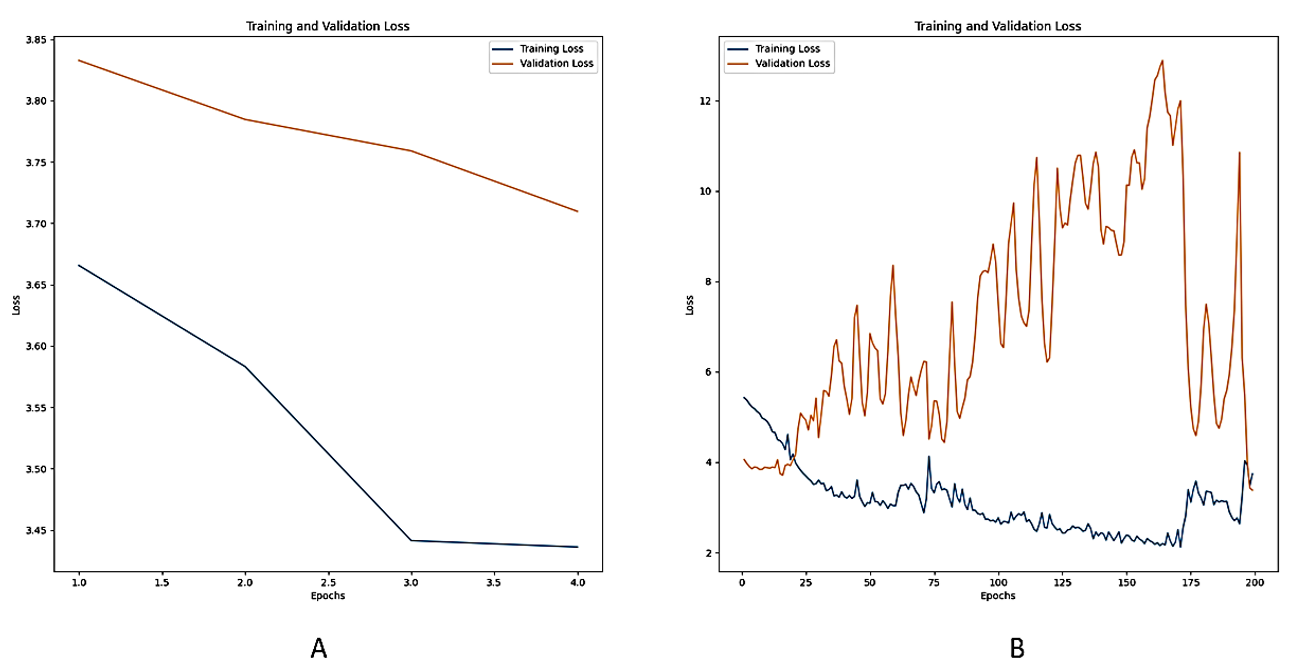
\includegraphics[width=0.98 \textwidth]{Images/fig2.png}
\vspace{-0.2cm}
\caption{\footnotesize{Training and validation loss curves indicating model convergence. 
Panel (A) illustrates the loss trajectory for the HF-related mortality model, and Panel (B) displays the trajectory for non-HF mortality. }}\label{fig2}
\end{center}
\end{figure}

\section*{Discussion and Conclusion}
In this study, we developed and evaluated a DLCR model to predict cause-specific mortality in patients with HF. The proposed model demonstrated satisfactory discriminative ability for both HF-related death and mortality due to other causes. Notably, predictive performance was higher for non-HF mortality (C-index = 0.81) compared with HF-related mortality (C-index = 0.71), indicating that the model effectively captures distinct risk patterns associated with competing outcomes.

These findings align with previous studies highlighting the potential of DL approaches in cardiovascular risk prediction. Earlier research has reported strong predictive performance of deep neural networks in HF prognosis and cardiovascular outcome prediction \cite{mall2023, singh2024}. In addition, conventional machine learning methods, including logistic regression and support vector machines, have been applied to identify high-risk individuals in clinical populations \cite{ozbaykarakus2022, krishnendu2024}. However, many of these approaches do not explicitly account for competing risks, which may lead to biased risk estimation in conditions such as HF where multiple causes of death coexist. By incorporating a competing risks framework, the proposed model provides a more appropriate representation of the underlying survival process.

The stronger predictive performance observed for non-HF mortality may reflect differences in the underlying predictors associated with each outcome or greater separability of risk profiles for these events within the dataset. Furthermore, the systematic hyperparameter tuning process, together with validation monitoring and checkpointing during training, likely contributed to the stability and robustness of the final model.

Several limitations should be considered. First, the retrospective nature of the study may introduce potential sources of bias. Second, the model was developed using data from a single tertiary cardiovascular center, which may limit generalizability to other populations. Future studies incorporating larger multicenter datasets and external validation are necessary to further assess the model's robustness and clinical applicability.

Overall, the proposed DLCR framework provides a promising approach for cause-specific risk prediction in HF patients and highlights the potential value of DL–based survival models in cardiovascular prognostic research.

In conclusion, the proposed deep learning–based competing risks model demonstrated effective performance in predicting cause-specific mortality among patients with heart failure. By accounting for competing outcomes, the model provides a more accurate framework for risk stratification compared with conventional approaches that ignore competing risks. The results highlight the potential of deep learning methods to capture complex clinical patterns and improve prognostic modeling in cardiovascular research. Future studies with larger, multicenter datasets and external validation are warranted to further confirm the clinical applicability of this approach.

%%%%%%%%%%%%%%%%%%%%%%%% References %%%%%%%%%%%%%%%%%%%%%%%%%%%%%
\begin{thebibliography}{9}

\bibitem[Sarteschi et al. (2020)]{sarteschi2020}
Sarteschi C., Souza W. V. d., Medeiros C., Oliveira P. S. R., Martins S. M., and Cesse E. A. P. (2020),
Predictors of post-discharge 30-day hospital readmission in decompensated heart failure patients,
{\it International Journal of Cardiovascular Sciences} 33, 175--184.

\bibitem[Virani et al. (2021)]{virani2021}
Virani S. S., Alonso A., Aparicio H. J., Benjamin E. J., Bittencourt M. S., Callaway C. W., et al. (2021),
Heart disease and stroke statistics-2021 update: a report from the American Heart Association,
{\it Circulation} 143(8), CIR0000000000000950.

\bibitem[Huang and Liu (2020)]{huang2020}
Huang P. and Liu Y. (2020),
Deepcompete: A deep learning approach to competing risks in continuous time domain,
{\it AMIA Annual Symposium Proceedings}, American Medical Informatics Association.

\bibitem[Gui and Li (2005)]{gui2005}
Gui J. and Li H. (2005),
Penalized Cox regression analysis in the high-dimensional and low-sample size settings, with applications to microarray gene expression data,
{\it Bioinformatics} 21(13), 3001--3008.

\bibitem[e Silva et al. (2022)]{esilva2022}
e Silva C. G. d. S., Buginga G. C., e Silva E. A. d. S., Arena R., Rouleau C. R., Aggarwal S., et al. (2022),
Prediction of mortality in coronary artery disease: role of machine learning and maximal exercise capacity,
{\it Mayo Clinic Proceedings}, Elsevier.

\bibitem[Lee C. et al. (2019)]{lee2019}
Lee C., Yoon J., Van Der Schaar M. (2019), Dynamic-deephit: A deep learning approach for dynamic survival analysis with competing risks based on longitudinal data, {\it IEEE Transactions on Biomedical Engineering}, 67(1):122-33.

\bibitem[Blumenstock et al. (2022)]{blumenstock2022}
Blumenstock G., Lessmann S., and Seow H.-V. (2022),
Deep learning for survival and competing risk modelling,
{\it Journal of the Operational Research Society} 73(1), 26--38.

\bibitem[Bellazzi et al. (2022)]{bellazzi2022}
Bellazzi R., Dagliati A., and Nicora G. (2022),
Predicting Medical Outcomes,
In: {\it Intelligent Systems in Medicine and Health: The Role of AI}, Springer, 309--342.

\bibitem[Fine J. P. and Gray R. J. (1999)]{fine1999}
Fine JP, Gray RJ, A proportional hazards model for the subdistribution of a competing risk (1999), {\it Journal of the American statistical association}, 94(446):496-509. 

\bibitem[Mall and Singh (2023)]{mall2023}
Mall S. and Singh J. (2023),
Comparative Study of Heart Failure Using the Approach of Machine Learning and Deep Neural Networks,
In: {\it International Conference on Data Analytics \& Management}, Springer.

\bibitem[Singh et al. (2024)]{singh2024}
Singh M. S., Thongam K., Choudhary P., and Bhagat P. (2024),
An Integrated Machine Learning Approach for Congestive Heart Failure Prediction,
{\it Diagnostics} 14(7), 736.

\bibitem[Özbay Karakuş and Er (2022)]{ozbaykarakus2022}
Özbay Karakuş M. and Er O. (2022),
A comparative study on prediction of survival event of heart failure patients using machine learning algorithms,
{\it Neural Computing and Applications} 34(16), 13895--13908.

\bibitem[Krishnendu et al. (2024)]{krishnendu2024}
Krishnendu S., Sarath S., Niveditha S., and Sai B. M. S. (2024),
Heart Failure Prediction using Machine Learning Techniques: A Comparative Analysis,
In: {\it 2024 15th International Conference on Computing Communication and Networking Technologies (ICCCNT)}, IEEE.

\end{thebibliography}
\end{document}